\documentclass[11pt,a4paper]{article}

\usepackage[utf8]{inputenc}
\usepackage[T1]{fontenc}
\usepackage[margin=2cm, headheight=15pt]{geometry}
\usepackage{graphicx}
\usepackage{xcolor}
\usepackage{amsmath,amssymb}
\usepackage{booktabs}
\usepackage{array}
\usepackage{listings}
\usepackage{hyperref}
\usepackage{fancyhdr}

% Palette de couleurs
\definecolor{inptblue}{HTML}{1E40AF}
\definecolor{inptlight}{HTML}{EFF6FF}
\definecolor{codebg}{HTML}{F8FAFC}
\definecolor{codeframe}{HTML}{CBD5E1}
\definecolor{codekw}{HTML}{1D4ED8}
\definecolor{codestr}{HTML}{15803D}
\definecolor{codecmt}{HTML}{64748B}
\definecolor{slate}{HTML}{334155}

\hypersetup{
    colorlinks=true,
    linkcolor=inptblue,
    urlcolor=inptblue,
    pdftitle={Architecture Logicielle et Explication du Code - IPv4 Subnet Toolkit v1.2.0},
    pdfauthor={INPT - Cursus Ingenieur ASEDS}
}

\pagestyle{fancy}
\fancyhf{}
\fancyhead[L]{\small\textbf{\textcolor{inptblue}{IPv4 Subnet Toolkit v1.2.0}} — Architecture \& Code}
\fancyhead[R]{\small\textcolor{slate}{Python / PyQt6 / Java OOP}}
\fancyfoot[C]{\thepage}

\setlength{\parskip}{0.55em}
\setlength{\parindent}{0pt}

% Configuration de listings pour Python et Java avec support des accents UTF-8
\lstset{
    backgroundcolor=\color{codebg},
    frame=single,
    rulecolor=\color{codeframe},
    basicstyle=\ttfamily\footnotesize,
    keywordstyle=\color{codekw}\bfseries,
    stringstyle=\color{codestr},
    commentstyle=\color{codecmt}\itshape,
    breaklines=true,
    showstringspaces=false,
    tabsize=4,
    captionpos=b,
    literate=
        {é}{{\'e}}1
        {è}{{\`e}}1
        {ê}{{\^e}}1
        {à}{{\`a}}1
        {ù}{{\`u}}1
        {û}{{\^u}}1
        {ô}{{\^o}}1
        {î}{{\^i}}1
        {ç}{{\c{c}}}1
        {É}{{\'E}}1
        {À}{{\`A}}1
        {→}{{$\rightarrow$}}1
        {≥}{{$\ge$}}1
        {−}{{$-$}}1
}

\newcommand{\techbox}[2]{%
    \vspace{0.4em}
    \noindent\fcolorbox{inptblue}{inptlight}{%
        \parbox{\dimexpr\linewidth-2\fboxsep-2\fboxrule\relax}{%
            \textbf{\textcolor{inptblue}{#1}}\\[0.3em]
            #2
        }%
    }%
    \vspace{0.4em}
}

\begin{document}

% ============================================================================
% PAGE DE TITRE
% ============================================================================
\begin{titlepage}
    \centering
    \vspace*{1.5cm}
    {\Large \textbf{\textcolor{inptblue}{INSTITUT NATIONAL DES POSTES ET TÉLÉCOMMUNICATIONS (INPT)}}}\\[0.3cm]
    {\large Cursus Ingénieur — Filière ASEDS}\\[2cm]

    \rule{\linewidth}{0.6mm}\\[0.5cm]
    {\Huge \textbf{\textcolor{inptblue}{IPv4 Subnet Toolkit v1.2.0}}}\\[0.4cm]
    {\LARGE \textbf{Architecture Logicielle, Ingénierie du Code Python/PyQt6 \& Blueprint de Portage Java OOP}}\\[0.3cm]
    \rule{\linewidth}{0.6mm}\\[1.2cm]

    {\large \textit{Explication complète du code source module par module : découplage Clean Architecture (\texttt{engine/} vs \texttt{ui/}), opérations binaires 32 bits, algorithmes des solveurs, événements clavier PyQt6, feuilles de style dynamiques QSS et compilation \texttt{.exe}.}}\\[1.5cm]

    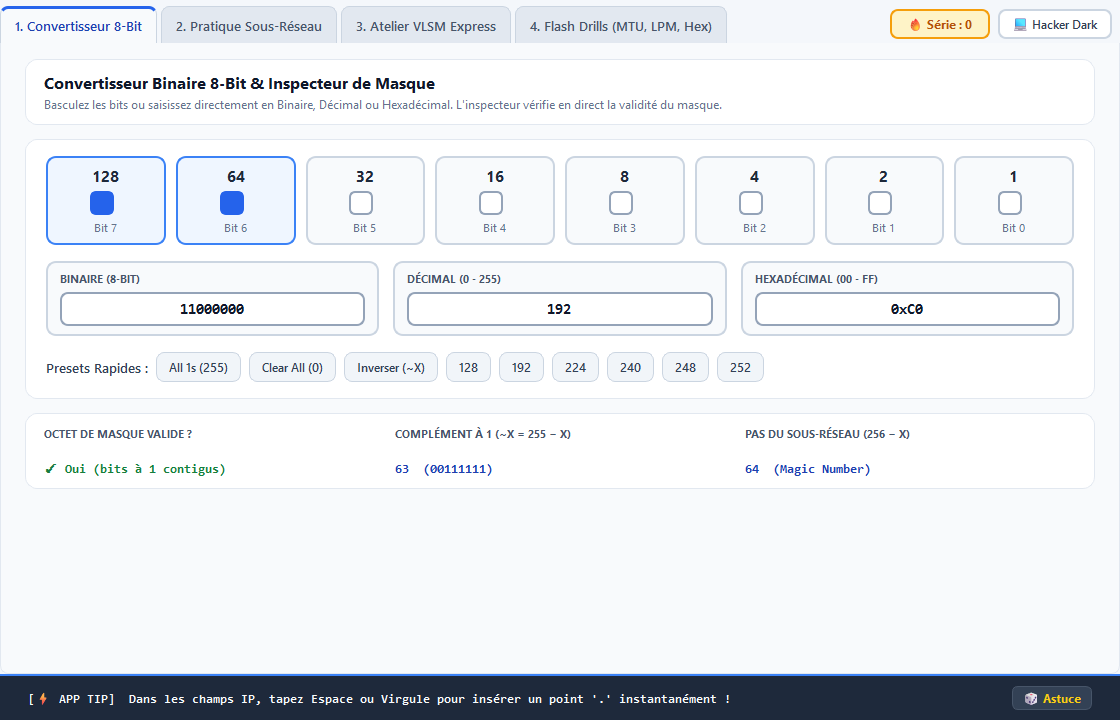
\includegraphics[width=0.92\textwidth]{../screenshots/01_tab1_mask_valid_light.png}\\[1.2cm]

    \vfill
    {\large \textbf{Version 1.2.0 — Octobre 2026}}\\
    {\normalsize Guide Technique \& Revue de Code Complète}
\end{titlepage}

\tableofcontents
\newpage

% ============================================================================
% CHAPITRE 1 : ARCHITECTURE GLOBALE & DECOUPLAGE MOTEUR / UI
% ============================================================================
\section{Architecture Globale : Du Monolithe v1.0.0 au Modèle Modulaire v1.2.0}

\subsection{Pourquoi Refactoriser l'Application en Deux Packages (\texttt{engine/} et \texttt{ui/}) ?}
Dans la version initiale \texttt{v1.0.0}, l'intégralité du programme (1\,171 lignes) résidait dans un seul fichier \texttt{converter.py} où les calculs d'adresses IP étaient exécutés directement à l'intérieur des callbacks des boutons PyQt6.

Pour la version \textbf{v1.2.0}, nous avons appliqué le patron d'architecture \textbf{Séparation des Préoccupations (\textit{Separation of Concerns — SoC})} :
\begin{itemize}
    \item \textbf{Le package \texttt{engine/} (Logique Métier Pure)} :
    Contient 100\,\% des mathématiques IPv4, de l'algorithme VLSM, des solveurs de fragmentation MTU, de routage LPM et de Checksum 16 bits. \textbf{Aucun fichier de \texttt{engine/} n'importe \texttt{PyQt6}}.
    \item \textbf{Le package \texttt{ui/} (Couche Présentation PyQt6)} :
    Ne contient aucune formule mathématique complexe. Les widgets graphiques délèguent chaque calcul à \texttt{engine/}, récupèrent un objet de données immuable (\texttt{@dataclass(frozen=True)}) et mettent à jour l'affichage.
\end{itemize}

\subsection{Arborescence Complète du Code Source v1.2.0}
\begin{lstlisting}
v1.2.0/
|-- converter.py                 # Point d'entree : instancie QApplication et MainWindow
|-- converter.exe                # Executable standalone compile via PyInstaller
|-- engine/                      # MOTEUR RESEAU PUR (100% Python standard, zero PyQt6)
|   |-- __init__.py              # Facade d'exportation du package engine
|   |-- ipv4_math.py             # Calculs d'octet, classes A-E, RFC1918, binaire 32 bits
|   |-- vlsm_solver.py           # Algorithme de decoupage VLSM & presets du cours INPT
|   |-- drills_solver.py         # Solveurs : Fragmentation MTU, Routage LPM, Checksum 16-bit
|   `-- tips_bank.py             # Banque de 16 astuces & gestionnaire de Serie / Progres
`-- ui/                          # INTERFACE GRAPHIQUE PYQT6
    |-- __init__.py
    |-- themes.py                # Feuilles de style QSS : Light Mode & Hacker Dark (#00FF66)
    |-- widgets.py               # IpLineEdit (auto-dot >= 26), MinecraftTipBanner, AdvancementToast
    |-- main_window.py           # Fenetre principale, barre d'onglets, Streak badge, Theme toggle
    |-- tab_binary.py            # Onglet 1 : Convertisseur 8-bit + Inspecteur de Masque
    |-- tab_subnet.py            # Onglet 2 : Pratique Sous-Reseau + Tiroir Binaire 32 bits
    |-- tab_vlsm.py              # Onglet 3 : Atelier VLSM Express avec auto-completion
    `-- tab_drills.py            # Onglet 4 : Flash Drills (QStackedWidget : MTU, LPM, Checksum)
\end{lstlisting}

\techbox{Avantage Majeur : Objets de Transfert Immuables (\texttt{@dataclass(frozen=True)})}{
Toutes les réponses renvoyées par \texttt{engine/} (\texttt{OctetAnalysis}, \texttt{SubnetAnalysis}, \texttt{VlsmAllocation}, \texttt{VlsmProblem}, \texttt{MtuProblem}, \texttt{LpmProblem}, \texttt{ChecksumProblem}) sont déclarées avec \texttt{@dataclass(frozen=True)}. Cela garantit que l'interface graphique ne peut jamais modifier accidentellement l'état interne d'un calcul, éliminant toute une catégorie de bugs d'effets de bord.
}

\newpage
% ============================================================================
% CHAPITRE 2 : EXPLICATION DU CODE DU MOTEUR (ENGINE/)
% ============================================================================
\section{Analyse Détaillée du Moteur Réseau (\texttt{engine/})}

\subsection{Module 1 : \texttt{engine/ipv4\_math.py} — Bitwise Math \& Sous-Réseaux 32 Bits}

\subsubsection{1. Inspection d'un Octet et Piège de l'Opérateur \texttt{$\sim$} en Python}
En Python, le type \texttt{int} a une précision arbitraire et est signé. L'opérateur d'inversion binaire \texttt{$\sim$val} calcule en réalité $-\text{val} - 1$ (complément à deux signé). Par exemple, $\sim 192 = -193$.
Pour obtenir le \textbf{complément à un non signé sur 8 bits} (ou sur 32 bits pour un masque complet), il est indispensable d'appliquer un masque bit à bit \texttt{\& 0xFF} (ou \texttt{\& 0xFFFFFFFF}) :

\begin{lstlisting}[language=Python, caption={Extrait de engine/ipv4\_math.py : Inspection d'un octet (0..255)}]
VALID_MASK_OCTETS: Tuple[int, ...] = (255, 254, 252, 248, 240, 224, 192, 128, 0)

class IPv4MathEngine:
    @staticmethod
    def is_valid_mask_octet(val: int) -> bool:
        """Vrai si l'octet possede des bits a 1 contigus de gauche a droite."""
        return val in VALID_MASK_OCTETS

    @staticmethod
    def ones_complement_octet(val: int) -> int:
        """Retourne le complement a 1 sur 8 bits (~val & 0xFF), soit 255 - val."""
        return (~val) & 0xFF

    @staticmethod
    def block_size_octet(val: int) -> int:
        """Retourne le pas du sous-reseau / Magic Number (256 - val)."""
        return 256 - max(0, min(255, val))
\end{lstlisting}

\subsubsection{2. Calcul Binaire 32 Bits de \texttt{Network}, \texttt{Host ID Interne} et \texttt{Broadcast}}
Dans la méthode \texttt{analyze\_subnet(ip\_str, cidr)}, nous convertissons l'adresse IPv4 en un entier 32 bits via \texttt{int(ipaddress.IPv4Address(ip\_str))}, puis nous construisons le masque 32 bits par décalage binaire à gauche :

\begin{lstlisting}[language=Python, caption={Extrait de engine/ipv4\_math.py : Opérations binaires 32 bits du cours}]
# Construction du masque 32 bits a partir du prefixe /CIDR
mask_int = ((0xFFFFFFFF << (32 - cidr)) & 0xFFFFFFFF) if cidr > 0 else 0
wildcard_int = (~mask_int) & 0xFFFFFFFF  # Complement a 1 du masque sur 32 bits

# Formules exactes du cours INPT :
network_int   = ip_int & mask_int         # Adresse Reseau = IP ET Masque
host_id_int   = ip_int & wildcard_int     # Host ID Interne = IP ET (~Masque)
broadcast_int = network_int | wildcard_int # Broadcast = Network OU (~Masque)

# Calcul des bits empruntes (b_S) et des bits d'hotes (b_H)
if default_cidr is not None and cidr >= default_cidr:
    borrowed_bits = cidr - default_cidr
    num_subnets = 1 << borrowed_bits      # 2^b_S sous-reseaux
else:
    borrowed_bits = 0
    num_subnets = 1

host_bits = 32 - cidr
usable_hosts = max(0, (1 << host_bits) - 2) # 2^b_H - 2 hotes disponibles
\end{lstlisting}
Remarquez l'utilisation de \texttt{1 << k} au lieu de \texttt{2 ** k} : en programmation système et réseau, le décalage binaire à gauche \texttt{1 << k} calcule exactement $2^k$ en une seule instruction processeur.

\subsubsection{3. Génération Aléatoire Pondérée (\texttt{generate\_practice\_problem})}
Dans \texttt{v1.0.0}, les octets étaient tirés uniformément au hasard, ce qui donnait 98\,\% d'adresses publiques et presque jamais d'adresses \texttt{Privées}, \texttt{APIPA} ou \texttt{Loopback}. En \texttt{v1.2.0}, \texttt{generate\_practice\_problem()} utilise une distribution de probabilité contrôlée (\texttt{random.random()}) :
\begin{itemize}
    \item 12\,\% de chance de générer une adresse \textbf{Loopback} (\texttt{127.x.x.x}, Classe A).
    \item 12\,\% de chance de générer une adresse \textbf{APIPA} (\texttt{169.254.x.x}, Classe B).
    \item 34\,\% de chance de générer une adresse \textbf{Privée RFC 1918} (\texttt{10.x.x.x}, \texttt{172.16..31.x.x}, ou \texttt{192.168.x.x}).
    \item 42\,\% de chance de générer une adresse \textbf{Publique} (Classe A, B ou C).
\end{itemize}
De plus, le \texttt{cidr} est toujours tiré dans l'intervalle $[\text{default\_cidr}, 30]$ pour que la formule du cours $b_S = \text{CIDR} - \text{default\_cidr}$ soit toujours applicable.

\newpage
\subsection{Module 2 : \texttt{engine/vlsm\_solver.py} — Algorithme de Découpage VLSM}

Le solveur VLSM implémente fidèlement la méthode vue en TD :
\begin{lstlisting}[language=Python, caption={Extrait de engine/vlsm\_solver.py : Dimensionnement et allocation séquentielle}]
class VlsmSolver:
    @staticmethod
    def smallest_host_bits(hosts_needed: int) -> int:
        """Trouve la plus petite puissance h >= 2 telle que 2^h - 2 >= hosts_needed."""
        if hosts_needed < 1:
            return 2
        h = max(2, math.ceil(math.log2(hosts_needed + 2)))
        while (1 << h) - 2 < hosts_needed:
            h += 1
        return h

    @classmethod
    def solve(cls, base_network_str: str, base_cidr: int, needs: List[int], title: str) -> VlsmProblem:
        base_net = ipaddress.IPv4Network(f"{base_network_str}/{base_cidr}", strict=False)
        current_ip_int = int(base_net.network_address)

        # Etape 1 : Tri strictement decroissant des besoins
        sorted_needs = sorted(needs, reverse=True)
        allocations: List[VlsmAllocation] = []

        # Etape 2 : Allocation sequentielle sans trou
        for idx, need in enumerate(sorted_needs, start=1):
            h = cls.smallest_host_bits(need)
            cidr = 32 - h
            block_size = 1 << h
            subnet = ipaddress.IPv4Network((current_ip_int, cidr), strict=False)
            ...
            # Avancer le pointeur d'adresse de la taille exacte du bloc (2^h)
            current_ip_int += block_size
\end{lstlisting}

\textbf{Pourquoi avancer simplement \texttt{current\_ip\_int += block\_size} fonctionne-t-il toujours ?}
Parce que \texttt{sorted\_needs} est trié par ordre décroissant, la suite des tailles de blocs $2^{h_1}, 2^{h_2}, 2^{h_3}$ est décroissante ($h_1 \ge h_2 \ge h_3$). Or, en arithmétique binaire, la somme $\text{Base} + 2^{h_1}$ (où $\text{Base}$ est alignée sur \texttt{/24}, donc multiple de $256$) est nécessairement divisible par $2^{h_2}$ dès lors que $h_2 \le h_1 \le 8$. Ainsi, chaque sous-réseau tombe exactement sur une frontière de masque valide !

\subsection{Module 3 : \texttt{engine/drills\_solver.py} — MTU, Routage LPM \& Checksum}

\begin{lstlisting}[language=Python, caption={Extrait de engine/drills\_solver.py : Fragmentation MTU et Checksum 16 bits}]
# 1. Alignement de la charge utile MTU sur un multiple de 8 octets :
header_len = ihl * 4
orig_data = max(0, total_length - header_len)
max_data = ((mtu - header_len) // 8) * 8

# 2. Somme de controle IPv4 (16 bits) avec rabattement iteratif de la retenue :
@staticmethod
def solve_checksum(words_hex: List[str], title: str = "") -> ChecksumProblem:
    cleaned_words = [w.strip().upper().replace("0X", "").zfill(4) for w in words_hex]
    raw_sum = sum(int(w, 16) for w in cleaned_words)

    carried = raw_sum
    while carried > 0xFFFF:
        carried = (carried & 0xFFFF) + (carried >> 16)

    checksum = (~carried) & 0xFFFF
    return ChecksumProblem(title, cleaned_words, raw_sum, carried, checksum)
\end{lstlisting}
\textbf{Détail subtil d'ingénierie} : Dans \texttt{solve\_checksum}, nous utilisons une boucle \texttt{while carried > 0xFFFF:} et non un simple \texttt{if}. En effet, si \texttt{raw\_sum} valait par exemple \texttt{0x1FFFF}, un seul rabattement donnerait $\texttt{0xFFFF} + \texttt{0x0001} = \texttt{0x10000}$, qui dépasse à nouveau \texttt{0xFFFF} ! La boucle \texttt{while} garantit que le résultat tient toujours sur 16 bits.

\newpage
% ============================================================================
% CHAPITRE 3 : INGENIERIE DE L'INTERFACE GRAPHIQUE PYQT6 (UI/)
% ============================================================================
\section{Ingénierie de l'Interface Graphique PyQt6 (\texttt{ui/})}

\subsection{Saisie Clavier Intelligente : \texttt{IpLineEdit} (\texttt{ui/widgets.py})}

Pour offrir une saisie ultra-fluide sans avoir à chercher la touche \texttt{.} sur le clavier, la classe \texttt{IpLineEdit} hérite de \texttt{QLineEdit} et redéfinit la méthode virtuelle \texttt{keyPressEvent(self, event: QKeyEvent)} :

\begin{lstlisting}[language=Python, caption={Code complet de IpLineEdit dans ui/widgets.py}]
class IpLineEdit(QLineEdit):
    def keyPressEvent(self, event):
        key = event.key()
        text = self.text()
        pos = self.cursorPosition()

        # 1. Espace ou Virgule insere un '.' ou saute par-dessus un '.' existant
        if key in (Qt.Key.Key_Space, Qt.Key.Key_Comma):
            if pos > 0 and text[pos - 1] not in ". ":
                if text.count(".") < 3:
                    self.insert(".")
                    return
            elif pos < len(text) and text[pos] == ".":
                self.setCursorPosition(pos + 1)
                return
            return

        # 2. Laisser QLineEdit traiter la frappe normale du caractere
        super().keyPressEvent(event)

        # 3. Lookahead mathematique : Auto-Dot apres 3 chiffres OU 2 chiffres >= 26
        if event.text().isdigit():
            cur_text = self.text()
            cur_pos = self.cursorPosition()
            if cur_pos == len(cur_text):
                last_dot = cur_text.rfind(".")
                last_space = cur_text.rfind(" ")
                sep = max(last_dot, last_space)
                octet = cur_text[sep + 1:] if sep != -1 else cur_text
                dots_count = cur_text.count(".") + cur_text.count(" ")

                if dots_count < 3 and octet.isdigit():
                    val = int(octet)
                    if len(octet) == 3 or (len(octet) == 2 and val >= 26):
                        self.insert(".")
\end{lstlisting}

\textbf{Pourquoi vérifier \texttt{event.text().isdigit()} après \texttt{super().keyPressEvent(event)} ?}
Si l'utilisateur appuie sur la touche \texttt{Backspace} pour effacer un point \texttt{.}, \texttt{event.text().isdigit()} vaut \texttt{False}. Ainsi, l'auto-dot ne se redéclenche jamais pendant un effacement, permettant de corriger librement sa saisie !

\subsection{Sélecteurs Dynamiques QSS et le Cycle \texttt{unpolish} / \texttt{polish}}

\begin{figure}[!htbp]
    \centering
    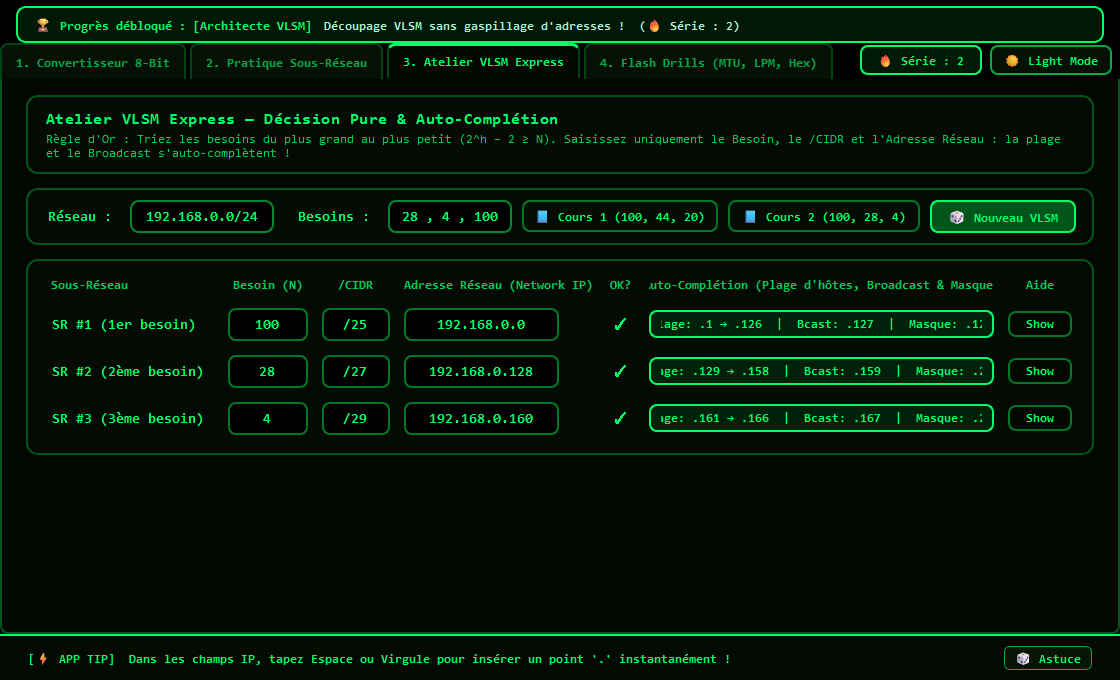
\includegraphics[width=0.92\textwidth]{../screenshots/06_tab3_vlsm_cours2_hacker.png}
    \caption{Rendu du thème \textbf{Hacker Dark} (\texttt{ui/themes.py}) sur l'onglet VLSM grâce aux propriétés dynamiques QSS.}
\end{figure}

Au lieu de modifier le style de chaque widget en Python avec des couleurs codées en dur (ce qui empêcherait de basculer proprement entre \textbf{Light Mode} et \textbf{Hacker Dark Mode}), nous utilisons des \textbf{propriétés dynamiques Qt} associées à des sélecteurs d'attributs dans \texttt{ui/themes.py} :
\begin{lstlisting}[caption={Extrait de ui/themes.py : Sélecteurs d'attributs QSS}]
#bitBox[active="true"] {
    background-color: #00220A;
    border: 2px solid #00FF66;
}
#choiceBtn[selected="true"] {
    background-color: #00FF66;
    border: 1.5px solid #00FF66;
    color: #000000;
}
#autoSummaryBadge[solved="true"] {
    border: 1.5px solid #00FF66;
    color: #00FF66;
    background-color: #00220A;
}
\end{lstlisting}

Dans le code Python (\texttt{tab\_binary.py}, \texttt{tab\_subnet.py}, \texttt{tab\_vlsm.py}, \texttt{tab\_drills.py}), lorsqu'un état change, on applique le pattern suivant :
\begin{lstlisting}[language=Python]
badge.setProperty("solved", True)
badge.style().unpolish(badge)
badge.style().polish(badge)
\end{lstlisting}
En Qt, \texttt{setProperty()} modifie l'attribut interne du \texttt{QObject}, mais le moteur de rendu CSS ne réévalue pas l'apparence tant qu'on n'appelle pas \texttt{unpolish()} suivi de \texttt{polish()}.

\subsection{Trois Patterns PyQt6 Essentiels Utilisés dans les Onglets}

\subsubsection{1. Le Verrou Anti-Récursion \texttt{self.\_updating} (\texttt{ui/tab\_binary.py})}
Dans l'onglet 1, modifier le champ Décimal met à jour les 8 cases à cocher, le champ Binaire et le champ Hexadécimal. Pour empêcher que le changement d'une case à cocher ne rappelle à son tour \texttt{on\_checkbox\_toggled()} en boucle infinie, \texttt{apply\_value()} encadre toutes les mises à jour avec \texttt{self.\_updating = True} dans un bloc \texttt{try...finally}, et ne réécrit pas dans le champ \texttt{source} en cours de frappe (préservant la position du curseur de l'utilisateur).

\subsubsection{2. La Subtilité \texttt{isHidden()} vs \texttt{isVisible()} (\texttt{ui/tab\_subnet.py})}
Pour ouvrir/fermer le tiroir binaire 32 bits, nous utilisons :
\begin{lstlisting}[language=Python]
def toggle_binary_drawer(self):
    vis = self.drawer_card.isHidden()
    self.drawer_card.setVisible(vis)
\end{lstlisting}
En PyQt6, \texttt{widget.isVisible()} retourne \texttt{False} si l'onglet parent n'est pas l'onglet actuellement affiché à l'écran, tandis que \texttt{widget.isHidden()} reflète l'état propre du tiroir indépendamment de l'onglet actif.

\subsubsection{3. Timers Asynchrones Non-Bloquants (\texttt{QTimer} dans \texttt{ui/widgets.py})}
\begin{itemize}
    \item \texttt{MinecraftTipBanner} utilise un \texttt{QTimer} périodique (\texttt{setInterval(12000)}) pour faire tourner les 16 astuces toutes les 12 secondes sur la boucle d'événements Qt sans jamais créer de thread secondaire ni utiliser \texttt{time.sleep()}.
    \item \texttt{AdvancementToast} utilise un \texttt{QTimer} \textit{single-shot} (\texttt{setSingleShot(True)}, \texttt{3200 ms}) qui masque automatiquement la bannière \texttt{Progrès débloqué !} au bout de 3,2 secondes.
\end{itemize}

\newpage
% ============================================================================
% CHAPITRE 4 : COMPILATION .EXE & BLUEPRINT DE PORTAGE JAVA OOP
% ============================================================================
\section{Compilation Standalone (\texttt{.exe}) \& Blueprint de Portage Java OOP}

\subsection{Fonctionnement de la Compilation PyInstaller (\texttt{converter.exe})}
L'exécutable autonome \texttt{v1.2.0/converter.exe} est généré via la commande :
\begin{lstlisting}
python -m PyInstaller --onefile --noconsole --name "converter" converter.py
\end{lstlisting}
\begin{itemize}
    \item \textbf{\texttt{--onefile}} : Empaquette l'interpréteur Python 3, les bibliothèques dynamiques Qt6 (\texttt{Qt6Core.dll}, \texttt{Qt6Gui.dll}, \texttt{Qt6Widgets.dll}) et nos packages \texttt{engine/} et \texttt{ui/} dans une archive compressée unique (\texttt{CArchive}).
    \item \textbf{\texttt{--noconsole}} : Utilise le bootloader Windows graphique (\texttt{runw.exe}) pour lancer directement la fenêtre PyQt6 sans ouvrir d'invite de commandes noire en arrière-plan.
\end{itemize}

\subsection{Blueprint de Portage vers Java Orienté Objet (Cursus ASEDS INPT)}
Grâce à l'isolation totale du dossier \texttt{engine/}, vous pouvez porter ce projet en \textbf{Java 17/21} (avec JavaFX ou Swing) en traduisant directement chaque module :

\subsubsection{1. Traduction des \texttt{@dataclass(frozen=True)} en \texttt{record} Java}
\begin{lstlisting}[language=Java, caption={Équivalent Java direct de OctetAnalysis et VlsmAllocation}]
package ma.inpt.aseds.subnet.engine;

public record OctetAnalysis(
    int value,
    String binaryStr,
    String hexStr,
    boolean isValidMaskOctet,
    int onesComplement,
    String onesComplementBinary,
    int blockSize
) {}
\end{lstlisting}

\subsubsection{2. Le Piège Critique en Java : \texttt{int} Signé 32 Bits vs \texttt{long} 64 Bits}
En Python, \texttt{0xFFFFFFFF} vaut $+4\,294\,967\,295$. En Java, le type \texttt{int} est signé sur 32 bits : \texttt{0xFFFFFFFF} vaut \texttt{-1}, et l'opérateur \texttt{>>} propage le bit de signe \texttt{1} à gauche !
Lors du portage Java de \texttt{IPv4MathEngine} et \texttt{DrillsSolver}, appliquez ces deux règles :
\begin{lstlisting}[language=Java, caption={Opérations binaires IPv4 sûres en Java}]
// Regle 1 : Utiliser long (64 bits) avec le suffixe L pour les masques 32 bits
long maskInt = (cidr > 0) ? ((0xFFFFFFFFL << (32 - cidr)) & 0xFFFFFFFFL) : 0L;
long wildcardInt = (~maskInt) & 0xFFFFFFFFL;
long networkInt = ipInt & maskInt;
long hostIdInt = ipInt & wildcardInt;
long broadcastInt = networkInt | wildcardInt;

// Regle 2 : Utiliser le decalage non signe >>> pour le Checksum 16 bits
int carried = rawSum;
while (carried > 0xFFFF) {
    carried = (carried & 0xFFFF) + (carried >>> 16);
}
int checksum = (~carried) & 0xFFFF;
\end{lstlisting}

\end{document}
